%% Font size %%
\documentclass[11pt]{article}

%% Load the custom package
\usepackage{Mathdoc}
\usetikzlibrary{calc}

%% Numéro de séquence %% Titre de la séquence %%
\renewcommand{\centerhead}{DS1 - Pythagore : Racines carrées, Arrondis, Hypoténuse}

%% Spacing commands %%
\renewcommand{\baselinestretch}{1} \setlength{\parindent}{0pt}

%% Encadré « Exemple traité »
\newenvironment{exempletraite}
{\begin{tcolorbox}[colback=white, colframe=black, boxrule=0.3mm,
    sharp corners, fonttitle=\bfseries, coltitle=black,
    colbacktitle=black!10, title={Exemple traité}]}
{\end{tcolorbox}}

%% Codage d'angle droit : sommet #1, voisins #2 et #3
\newcommand{\angledroit}[3]{%
  \draw ($(#1)!0.25cm!(#2)$) -- ($(#1)!0.25cm!(#2) + (#1)!0.25cm!(#3) - (#1)$)
  -- ($(#1)!0.25cm!(#3)$);}

%% Ligne de réponse dans un tableau
\newcommand{\rep}{\rule{0pt}{5ex}}

\begin{document}

\entetedevoirs{20}

\begin{center}
\coefficient{1}
\calculatrice{1}
\end{center}

%%%%%%%%%%%%%%%%%%%%%%%%%%%%%%%%%%%%%%%%%%%%%%%%%%%%%%%%%%%%%%%%%%%%%%%%
\begin{exercicedevoir}[3][Racines carrées à connaître]
Compléter. Ces racines carrées se calculent de tête : la calculatrice
ne sert qu'à vérifier.

\renewcommand{\arraystretch}{2.2}
\begin{center}
\begin{tabular}{llll}
$\sqrt{4} = \ldots\ldots$ & $\sqrt{9} = \ldots\ldots$ & $\sqrt{1} = \ldots\ldots$ & $\sqrt{25} = \ldots\ldots$ \\
$\sqrt{16} = \ldots\ldots$ & $\sqrt{49} = \ldots\ldots$ & $\sqrt{36} = \ldots\ldots$ & $\sqrt{81} = \ldots\ldots$ \\
$\sqrt{64} = \ldots\ldots$ & $\sqrt{100} = \ldots\ldots$ & $\sqrt{0} = \ldots\ldots$ & $\sqrt{144} = \ldots\ldots$ \\
$\sqrt{121} = \ldots\ldots$ & $\sqrt{196} = \ldots\ldots$ & $\sqrt{169} = \ldots\ldots$ & $\sqrt{225} = \ldots\ldots$ \\
\end{tabular}
\end{center}
\end{exercicedevoir}

%%%%%%%%%%%%%%%%%%%%%%%%%%%%%%%%%%%%%%%%%%%%%%%%%%%%%%%%%%%%%%%%%%%%%%%%
\begin{exercicedevoir}[4][Racines carrées de grands carrés]
\textbf{1.} À l'aide de la calculatrice, compléter.

\renewcommand{\arraystretch}{2.2}
\begin{center}
\begin{tabular}{llll}
$\sqrt{256} = \ldots\ldots$ & $\sqrt{289} = \ldots\ldots$ & $\sqrt{324} = \ldots\ldots$ & $\sqrt{361} = \ldots\ldots$ \\
$\sqrt{400} = \ldots\ldots$ & $\sqrt{484} = \ldots\ldots$ & $\sqrt{529} = \ldots\ldots$ & $\sqrt{625} = \ldots\ldots$ \\
\end{tabular}
\end{center}

\textbf{2.} Cette fois, c'est le résultat qui est donné : trouver le
nombre qui se cache sous la racine.

\textit{Exemple : $\sqrt{\ldots\ldots} = 5$ \quad se complète en \quad
  $\sqrt{25} = 5$ \quad car $5^2 = 25$.}

\begin{center}
\begin{tabular}{llll}
$\sqrt{\ldots\ldots} = 7$ & $\sqrt{\ldots\ldots} = 12$ & $\sqrt{\ldots\ldots} = 15$ & $\sqrt{\ldots\ldots} = 17$ \\
$\sqrt{\ldots\ldots} = 20$ & $\sqrt{\ldots\ldots} = 21$ & $\sqrt{\ldots\ldots} = 23$ & $\sqrt{\ldots\ldots} = 25$ \\
\end{tabular}
\end{center}
\end{exercicedevoir}

%%%%%%%%%%%%%%%%%%%%%%%%%%%%%%%%%%%%%%%%%%%%%%%%%%%%%%%%%%%%%%%%%%%%%%%%
\begin{exercicedevoir}[5][Arrondis]
\begin{exempletraite}
On veut \textbf{arrondir $0{,}25$ au dixième}.
\begin{itemize}
\item Le chiffre des dixièmes est \textbf{2} : $0{,}\underline{2}5$.
\item On regarde le chiffre \textbf{juste après} (ici le chiffre des
  centièmes) : c'est \textbf{5}.
\item S'il vaut 0, 1, 2, 3 ou 4 : on garde le chiffre des dixièmes. \\
  S'il vaut 5, 6, 7, 8 ou 9 : on ajoute 1 au chiffre des dixièmes.
\item Ici, $5$ : on ajoute 1, donc $2$ devient $3$. \\
  \textbf{L'arrondi de $0{,}25$ au dixième est $0{,}3$.}
\end{itemize}
Autre exemple : arrondir $3{,}141$ au centième. Le chiffre après les
centièmes est $1$, on garde : \textbf{$3{,}14$}.
\end{exempletraite}

Compléter le tableau en imitant la première ligne.

\renewcommand{\arraystretch}{1.3}
\begin{center}
\begin{tabular}{|c|c|p{6.5cm}|c|}
\hline
\textbf{Nombre} & \textbf{Arrondi au\ldots} & \textbf{Explication} &
\textbf{Arrondi} \\ \hline
$0{,}25$ & dixième & \textit{chiffre suivant : 5, j'ajoute 1} &
$0{,}3$ \\ \hline
$0{,}73$ & dixième & \rep & \\ \hline
$4{,}86$ & dixième & \rep & \\ \hline
$15{,}082$ & dixième & \rep & \\ \hline
$12{,}348$ & centième & \rep & \\ \hline
$7{,}6521$ & centième & \rep & \\ \hline
$2{,}4136$ & millième & \rep & \\ \hline
$0{,}5072$ & millième & \rep & \\ \hline
$3{,}7058$ & millième & \rep & \\ \hline
\end{tabular}
\end{center}
\end{exercicedevoir}

%%%%%%%%%%%%%%%%%%%%%%%%%%%%%%%%%%%%%%%%%%%%%%%%%%%%%%%%%%%%%%%%%%%%%%%%
\begin{exercicedevoir}[4][Arrondir une racine carrée]
\begin{exempletraite}
On veut \textbf{arrondir $\sqrt{30}$ au centième}.
\begin{enumerate}
\item Je calcule la racine à la calculatrice et j'écris plusieurs
  chiffres après la virgule : $\sqrt{30} = 5{,}4772\ldots$
\item J'arrondis au centième : le chiffre après les centièmes est
  $7$, j'ajoute 1. \\
  \textbf{$\sqrt{30} \approx 5{,}48$ (arrondi au centième).}
\end{enumerate}
\end{exempletraite}

Compléter le tableau en imitant la première ligne.

\renewcommand{\arraystretch}{1.3}
\begin{center}
\begin{tabular}{|c|c|p{4.5cm}|p{3cm}|}
\hline
\textbf{Racine} & \textbf{Arrondi au\ldots} &
\textbf{Calculatrice (4 chiffres après la virgule)} & \textbf{Arrondi} \\ \hline
$\sqrt{30}$ & centième & $5{,}4772\ldots$ & $5{,}48$ \\ \hline
$\sqrt{2}$ & dixième & \rep & \\ \hline
$\sqrt{50}$ & dixième & \rep & \\ \hline
$\sqrt{10}$ & centième & \rep & \\ \hline
$\sqrt{45}$ & centième & \rep & \\ \hline
$\sqrt{12}$ & millième & \rep & \\ \hline
$\sqrt{7}$ & millième & \rep & \\ \hline
\end{tabular}
\end{center}
\end{exercicedevoir}

%%%%%%%%%%%%%%%%%%%%%%%%%%%%%%%%%%%%%%%%%%%%%%%%%%%%%%%%%%%%%%%%%%%%%%%%
\begin{exercicedevoir}[4][Hypoténuse]
Pour chaque triangle rectangle, écrire le nom de son hypoténuse.

\vspace{0.5em}
\begin{minipage}[b]{0.24\linewidth}
\centering
\begin{tikzpicture}
\coordinate (F) at (0,0); \coordinate (E) at (0,2.2);
\coordinate (G) at (2.8,0);
\draw (E) -- (F) -- (G) -- cycle; \angledroit{F}{E}{G}
\node[above] at (E) {$E$}; \node[below left] at (F) {$F$};
\node[below right] at (G) {$G$};
\end{tikzpicture}

\vspace{0.5em}
Triangle $EFG$ rectangle en $F$.

\vspace{0.8em}
Hypoténuse : \ldots\ldots\ldots
\end{minipage}%
\hfill
\begin{minipage}[b]{0.24\linewidth}
\centering
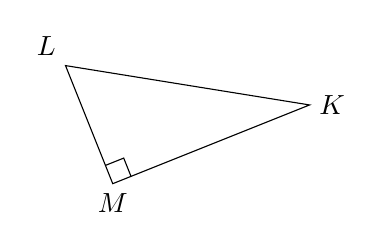
\begin{tikzpicture}
\coordinate (M) at (0,0); \coordinate (K) at (2.5,1);
\coordinate (L) at (-0.6,1.5);
\draw (K) -- (L) -- (M) -- cycle; \angledroit{M}{K}{L}
\node[below] at (M) {$M$}; \node[right] at (K) {$K$};
\node[above left] at (L) {$L$};
\end{tikzpicture}

\vspace{0.5em}
Triangle $KLM$ rectangle en $M$.

\vspace{0.8em}
Hypoténuse : \ldots\ldots\ldots
\end{minipage}%
\hfill
\begin{minipage}[b]{0.24\linewidth}
\centering
\begin{tikzpicture}
\coordinate (R) at (1.2,2); \coordinate (S) at (0,0);
\coordinate (T) at (3.4,0.68);
\draw (R) -- (S) -- (T) -- cycle; \angledroit{R}{S}{T}
\node[above] at (R) {$R$}; \node[below left] at (S) {$S$};
\node[right] at (T) {$T$};
\end{tikzpicture}

\vspace{0.5em}
Triangle $RST$ rectangle en $R$.

\vspace{0.8em}
Hypoténuse : \ldots\ldots\ldots
\end{minipage}%
\hfill
\begin{minipage}[b]{0.24\linewidth}
\centering
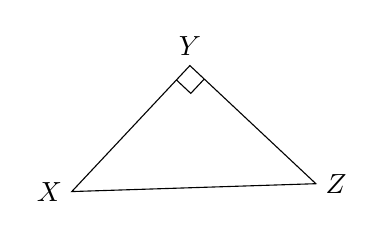
\begin{tikzpicture}
\coordinate (Y) at (1.5,2.2); \coordinate (X) at (0,0.6);
\coordinate (Z) at (3.1,0.7);
\draw (X) -- (Y) -- (Z) -- cycle; \angledroit{Y}{X}{Z}
\node[above] at (Y) {$Y$}; \node[left] at (X) {$X$};
\node[right] at (Z) {$Z$};
\end{tikzpicture}

\vspace{0.5em}
Triangle $XYZ$ rectangle en $Y$.

\vspace{0.8em}
Hypoténuse : \ldots\ldots\ldots
\end{minipage}
\end{exercicedevoir}

\end{document}

%%% Local Variables:
%%% mode: LaTeX
%%% TeX-master: t
%%% End:
